\tikzset{every picture/.style={line width=0.75pt}} %set default line width to 0.75pt        

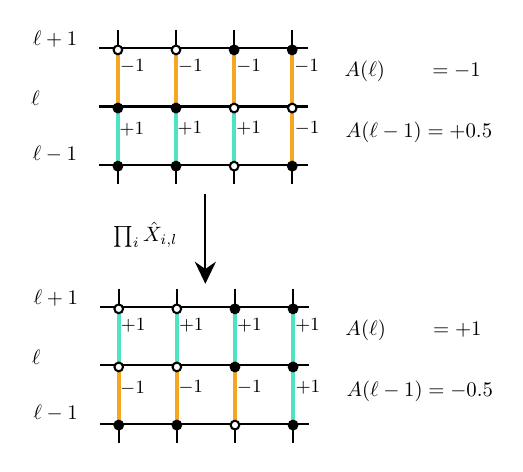
\begin{tikzpicture}[x=0.75pt,y=0.75pt,yscale=-1,xscale=1]
%uncomment if require: \path (0,300); %set diagram left start at 0, and has height of 300

%Shape: Grid [id:dp9360441110029474] 
\draw  [draw opacity=0] (257.87,63.33) -- (358.47,63.33) -- (358.47,137.8) -- (257.87,137.8) -- cycle ; \draw   (266.87,63.33) -- (266.87,137.8)(294.87,63.33) -- (294.87,137.8)(322.87,63.33) -- (322.87,137.8)(350.87,63.33) -- (350.87,137.8) ; \draw   (257.87,72.33) -- (358.47,72.33)(257.87,100.33) -- (358.47,100.33)(257.87,128.33) -- (358.47,128.33) ; \draw    ;
%Straight Lines [id:da29151561133025305] 
\draw [color={rgb, 255:red, 245; green, 166; blue, 35 }  ,draw opacity=1 ][line width=1.5]    (266.87,75.17) -- (266.87,98.96) ;
%Straight Lines [id:da4446819281500063] 
\draw [color={rgb, 255:red, 245; green, 166; blue, 35 }  ,draw opacity=1 ][line width=1.5]    (294.87,75.17) -- (294.87,98.96) ;
%Straight Lines [id:da07715323952982911] 
\draw [color={rgb, 255:red, 245; green, 166; blue, 35 }  ,draw opacity=1 ][line width=1.5]    (322.87,75.17) -- (322.87,98.96) ;
%Straight Lines [id:da9182453323662629] 
\draw [color={rgb, 255:red, 245; green, 166; blue, 35 }  ,draw opacity=1 ][line width=1.5]    (350.87,75.17) -- (350.87,98.96) ;
%Straight Lines [id:da8352991049825591] 
\draw [color={rgb, 255:red, 245; green, 166; blue, 35 }  ,draw opacity=1 ][line width=1.5]    (350.87,103.17) -- (350.87,126.96) ;
%Straight Lines [id:da5440682265060037] 
\draw [color={rgb, 255:red, 80; green, 227; blue, 194 }  ,draw opacity=1 ][line width=1.5]    (266.87,103.17) -- (266.87,126.96) ;
%Straight Lines [id:da13028385723345526] 
\draw [color={rgb, 255:red, 80; green, 227; blue, 194 }  ,draw opacity=1 ][line width=1.5]    (294.87,103.17) -- (294.87,126.96) ;
%Straight Lines [id:da6808974953785236] 
\draw [color={rgb, 255:red, 80; green, 227; blue, 194 }  ,draw opacity=1 ][line width=1.5]    (322.87,103.17) -- (322.87,126.96) ;
%Shape: Ellipse [id:dp1850047692569765] 
\draw  [color={rgb, 255:red, 0; green, 0; blue, 0 }  ,draw opacity=1 ][fill={rgb, 255:red, 0; green, 0; blue, 0 }  ,fill opacity=1 ] (320.8,73.07) .. controls (320.8,71.9) and (321.72,70.96) .. (322.87,70.96) .. controls (324.01,70.96) and (324.94,71.9) .. (324.94,73.07) .. controls (324.94,74.23) and (324.01,75.17) .. (322.87,75.17) .. controls (321.72,75.17) and (320.8,74.23) .. (320.8,73.07) -- cycle ;
%Shape: Ellipse [id:dp2682566882997268] 
\draw  [color={rgb, 255:red, 0; green, 0; blue, 0 }  ,draw opacity=1 ][fill={rgb, 255:red, 255; green, 255; blue, 255 }  ,fill opacity=1 ] (348.8,101.07) .. controls (348.8,99.9) and (349.72,98.96) .. (350.87,98.96) .. controls (352.01,98.96) and (352.94,99.9) .. (352.94,101.07) .. controls (352.94,102.23) and (352.01,103.17) .. (350.87,103.17) .. controls (349.72,103.17) and (348.8,102.23) .. (348.8,101.07) -- cycle ;
%Shape: Ellipse [id:dp09070102556660964] 
\draw  [color={rgb, 255:red, 0; green, 0; blue, 0 }  ,draw opacity=1 ][fill={rgb, 255:red, 0; green, 0; blue, 0 }  ,fill opacity=1 ] (348.8,73.07) .. controls (348.8,71.9) and (349.72,70.96) .. (350.87,70.96) .. controls (352.01,70.96) and (352.94,71.9) .. (352.94,73.07) .. controls (352.94,74.23) and (352.01,75.17) .. (350.87,75.17) .. controls (349.72,75.17) and (348.8,74.23) .. (348.8,73.07) -- cycle ;
%Shape: Ellipse [id:dp04233795078816582] 
\draw  [color={rgb, 255:red, 0; green, 0; blue, 0 }  ,draw opacity=1 ][fill={rgb, 255:red, 255; green, 255; blue, 255 }  ,fill opacity=1 ] (320.8,101.07) .. controls (320.8,99.9) and (321.72,98.96) .. (322.87,98.96) .. controls (324.01,98.96) and (324.94,99.9) .. (324.94,101.07) .. controls (324.94,102.23) and (324.01,103.17) .. (322.87,103.17) .. controls (321.72,103.17) and (320.8,102.23) .. (320.8,101.07) -- cycle ;
%Shape: Ellipse [id:dp5323178578796932] 
\draw  [color={rgb, 255:red, 0; green, 0; blue, 0 }  ,draw opacity=1 ][fill={rgb, 255:red, 0; green, 0; blue, 0 }  ,fill opacity=1 ] (348.8,129.07) .. controls (348.8,127.9) and (349.72,126.96) .. (350.87,126.96) .. controls (352.01,126.96) and (352.94,127.9) .. (352.94,129.07) .. controls (352.94,130.23) and (352.01,131.17) .. (350.87,131.17) .. controls (349.72,131.17) and (348.8,130.23) .. (348.8,129.07) -- cycle ;
%Shape: Ellipse [id:dp1503569502976856] 
\draw  [color={rgb, 255:red, 0; green, 0; blue, 0 }  ,draw opacity=1 ][fill={rgb, 255:red, 255; green, 255; blue, 255 }  ,fill opacity=1 ] (320.8,129.07) .. controls (320.8,127.9) and (321.72,126.96) .. (322.87,126.96) .. controls (324.01,126.96) and (324.94,127.9) .. (324.94,129.07) .. controls (324.94,130.23) and (324.01,131.17) .. (322.87,131.17) .. controls (321.72,131.17) and (320.8,130.23) .. (320.8,129.07) -- cycle ;
%Shape: Ellipse [id:dp02677782293641595] 
\draw  [color={rgb, 255:red, 0; green, 0; blue, 0 }  ,draw opacity=1 ][fill={rgb, 255:red, 0; green, 0; blue, 0 }  ,fill opacity=1 ] (292.8,129.07) .. controls (292.8,127.9) and (293.72,126.96) .. (294.87,126.96) .. controls (296.01,126.96) and (296.94,127.9) .. (296.94,129.07) .. controls (296.94,130.23) and (296.01,131.17) .. (294.87,131.17) .. controls (293.72,131.17) and (292.8,130.23) .. (292.8,129.07) -- cycle ;
%Shape: Ellipse [id:dp491912283653837] 
\draw  [color={rgb, 255:red, 0; green, 0; blue, 0 }  ,draw opacity=1 ][fill={rgb, 255:red, 0; green, 0; blue, 0 }  ,fill opacity=1 ] (292.8,101.07) .. controls (292.8,99.9) and (293.72,98.96) .. (294.87,98.96) .. controls (296.01,98.96) and (296.94,99.9) .. (296.94,101.07) .. controls (296.94,102.23) and (296.01,103.17) .. (294.87,103.17) .. controls (293.72,103.17) and (292.8,102.23) .. (292.8,101.07) -- cycle ;
%Shape: Ellipse [id:dp6499714395045919] 
\draw  [color={rgb, 255:red, 0; green, 0; blue, 0 }  ,draw opacity=1 ][fill={rgb, 255:red, 255; green, 255; blue, 255 }  ,fill opacity=1 ] (292.8,73.07) .. controls (292.8,71.9) and (293.72,70.96) .. (294.87,70.96) .. controls (296.01,70.96) and (296.94,71.9) .. (296.94,73.07) .. controls (296.94,74.23) and (296.01,75.17) .. (294.87,75.17) .. controls (293.72,75.17) and (292.8,74.23) .. (292.8,73.07) -- cycle ;
%Shape: Ellipse [id:dp1355435857945937] 
\draw  [color={rgb, 255:red, 0; green, 0; blue, 0 }  ,draw opacity=1 ][fill={rgb, 255:red, 0; green, 0; blue, 0 }  ,fill opacity=1 ] (264.8,129.07) .. controls (264.8,127.9) and (265.72,126.96) .. (266.87,126.96) .. controls (268.01,126.96) and (268.94,127.9) .. (268.94,129.07) .. controls (268.94,130.23) and (268.01,131.17) .. (266.87,131.17) .. controls (265.72,131.17) and (264.8,130.23) .. (264.8,129.07) -- cycle ;
%Shape: Ellipse [id:dp055580278077323575] 
\draw  [color={rgb, 255:red, 0; green, 0; blue, 0 }  ,draw opacity=1 ][fill={rgb, 255:red, 0; green, 0; blue, 0 }  ,fill opacity=1 ] (264.8,101.07) .. controls (264.8,99.9) and (265.72,98.96) .. (266.87,98.96) .. controls (268.01,98.96) and (268.94,99.9) .. (268.94,101.07) .. controls (268.94,102.23) and (268.01,103.17) .. (266.87,103.17) .. controls (265.72,103.17) and (264.8,102.23) .. (264.8,101.07) -- cycle ;
%Shape: Ellipse [id:dp12069303908542639] 
\draw  [color={rgb, 255:red, 0; green, 0; blue, 0 }  ,draw opacity=1 ][fill={rgb, 255:red, 255; green, 255; blue, 255 }  ,fill opacity=1 ] (264.8,73.07) .. controls (264.8,71.9) and (265.72,70.96) .. (266.87,70.96) .. controls (268.01,70.96) and (268.94,71.9) .. (268.94,73.07) .. controls (268.94,74.23) and (268.01,75.17) .. (266.87,75.17) .. controls (265.72,75.17) and (264.8,74.23) .. (264.8,73.07) -- cycle ;
%Shape: Grid [id:dp5018368968714211] 
\draw  [draw opacity=0] (258.27,188.08) -- (358.87,188.08) -- (358.87,262.55) -- (258.27,262.55) -- cycle ; \draw   (267.27,188.08) -- (267.27,262.55)(295.27,188.08) -- (295.27,262.55)(323.27,188.08) -- (323.27,262.55)(351.27,188.08) -- (351.27,262.55) ; \draw   (258.27,197.08) -- (358.87,197.08)(258.27,225.08) -- (358.87,225.08)(258.27,253.08) -- (358.87,253.08) ; \draw    ;
%Straight Lines [id:da559777946591173] 
\draw [color={rgb, 255:red, 80; green, 227; blue, 194 }  ,draw opacity=1 ][line width=1.5]    (267.27,199.92) -- (267.27,223.71) ;
%Straight Lines [id:da8649803187484479] 
\draw [color={rgb, 255:red, 80; green, 227; blue, 194 }  ,draw opacity=1 ][line width=1.5]    (295.27,199.92) -- (295.27,223.71) ;
%Straight Lines [id:da19427387583895772] 
\draw [color={rgb, 255:red, 80; green, 227; blue, 194 }  ,draw opacity=1 ][line width=1.5]    (323.27,199.92) -- (323.27,223.71) ;
%Straight Lines [id:da11966513957053504] 
\draw [color={rgb, 255:red, 80; green, 227; blue, 194 }  ,draw opacity=1 ][line width=1.5]    (351.27,199.92) -- (351.27,223.71) ;
%Straight Lines [id:da0046060300455432746] 
\draw [color={rgb, 255:red, 80; green, 227; blue, 194 }  ,draw opacity=1 ][line width=1.5]    (351.27,227.92) -- (351.27,251.71) ;
%Straight Lines [id:da05482936721591858] 
\draw [color={rgb, 255:red, 245; green, 166; blue, 35 }  ,draw opacity=1 ][line width=1.5]    (267.27,227.92) -- (267.27,251.71) ;
%Straight Lines [id:da7333488113220632] 
\draw [color={rgb, 255:red, 245; green, 166; blue, 35 }  ,draw opacity=1 ][line width=1.5]    (295.27,227.92) -- (295.27,251.71) ;
%Straight Lines [id:da19210010981044467] 
\draw [color={rgb, 255:red, 245; green, 166; blue, 35 }  ,draw opacity=1 ][line width=1.5]    (323.27,227.92) -- (323.27,251.71) ;
%Shape: Ellipse [id:dp0056932623931387205] 
\draw  [color={rgb, 255:red, 0; green, 0; blue, 0 }  ,draw opacity=1 ][fill={rgb, 255:red, 0; green, 0; blue, 0 }  ,fill opacity=1 ] (321.2,197.82) .. controls (321.2,196.65) and (322.12,195.71) .. (323.27,195.71) .. controls (324.41,195.71) and (325.34,196.65) .. (325.34,197.82) .. controls (325.34,198.98) and (324.41,199.92) .. (323.27,199.92) .. controls (322.12,199.92) and (321.2,198.98) .. (321.2,197.82) -- cycle ;
%Shape: Ellipse [id:dp9108217775135579] 
\draw  [color={rgb, 255:red, 0; green, 0; blue, 0 }  ,draw opacity=1 ][fill={rgb, 255:red, 0; green, 0; blue, 0 }  ,fill opacity=1 ] (349.2,225.82) .. controls (349.2,224.65) and (350.12,223.71) .. (351.27,223.71) .. controls (352.41,223.71) and (353.34,224.65) .. (353.34,225.82) .. controls (353.34,226.98) and (352.41,227.92) .. (351.27,227.92) .. controls (350.12,227.92) and (349.2,226.98) .. (349.2,225.82) -- cycle ;
%Shape: Ellipse [id:dp6920254647091042] 
\draw  [color={rgb, 255:red, 0; green, 0; blue, 0 }  ,draw opacity=1 ][fill={rgb, 255:red, 0; green, 0; blue, 0 }  ,fill opacity=1 ] (349.2,197.82) .. controls (349.2,196.65) and (350.12,195.71) .. (351.27,195.71) .. controls (352.41,195.71) and (353.34,196.65) .. (353.34,197.82) .. controls (353.34,198.98) and (352.41,199.92) .. (351.27,199.92) .. controls (350.12,199.92) and (349.2,198.98) .. (349.2,197.82) -- cycle ;
%Shape: Ellipse [id:dp9959333720441377] 
\draw  [color={rgb, 255:red, 0; green, 0; blue, 0 }  ,draw opacity=1 ][fill={rgb, 255:red, 0; green, 0; blue, 0 }  ,fill opacity=1 ] (321.2,225.82) .. controls (321.2,224.65) and (322.12,223.71) .. (323.27,223.71) .. controls (324.41,223.71) and (325.34,224.65) .. (325.34,225.82) .. controls (325.34,226.98) and (324.41,227.92) .. (323.27,227.92) .. controls (322.12,227.92) and (321.2,226.98) .. (321.2,225.82) -- cycle ;
%Shape: Ellipse [id:dp4611789257362229] 
\draw  [color={rgb, 255:red, 0; green, 0; blue, 0 }  ,draw opacity=1 ][fill={rgb, 255:red, 0; green, 0; blue, 0 }  ,fill opacity=1 ] (349.2,253.82) .. controls (349.2,252.65) and (350.12,251.71) .. (351.27,251.71) .. controls (352.41,251.71) and (353.34,252.65) .. (353.34,253.82) .. controls (353.34,254.98) and (352.41,255.92) .. (351.27,255.92) .. controls (350.12,255.92) and (349.2,254.98) .. (349.2,253.82) -- cycle ;
%Shape: Ellipse [id:dp7876740998470513] 
\draw  [color={rgb, 255:red, 0; green, 0; blue, 0 }  ,draw opacity=1 ][fill={rgb, 255:red, 255; green, 255; blue, 255 }  ,fill opacity=1 ] (321.2,253.82) .. controls (321.2,252.65) and (322.12,251.71) .. (323.27,251.71) .. controls (324.41,251.71) and (325.34,252.65) .. (325.34,253.82) .. controls (325.34,254.98) and (324.41,255.92) .. (323.27,255.92) .. controls (322.12,255.92) and (321.2,254.98) .. (321.2,253.82) -- cycle ;
%Shape: Ellipse [id:dp10449786736501454] 
\draw  [color={rgb, 255:red, 0; green, 0; blue, 0 }  ,draw opacity=1 ][fill={rgb, 255:red, 0; green, 0; blue, 0 }  ,fill opacity=1 ] (293.2,253.82) .. controls (293.2,252.65) and (294.12,251.71) .. (295.27,251.71) .. controls (296.41,251.71) and (297.34,252.65) .. (297.34,253.82) .. controls (297.34,254.98) and (296.41,255.92) .. (295.27,255.92) .. controls (294.12,255.92) and (293.2,254.98) .. (293.2,253.82) -- cycle ;
%Shape: Ellipse [id:dp31866222758058504] 
\draw  [color={rgb, 255:red, 0; green, 0; blue, 0 }  ,draw opacity=1 ][fill={rgb, 255:red, 255; green, 255; blue, 255 }  ,fill opacity=1 ] (293.2,225.82) .. controls (293.2,224.65) and (294.12,223.71) .. (295.27,223.71) .. controls (296.41,223.71) and (297.34,224.65) .. (297.34,225.82) .. controls (297.34,226.98) and (296.41,227.92) .. (295.27,227.92) .. controls (294.12,227.92) and (293.2,226.98) .. (293.2,225.82) -- cycle ;
%Shape: Ellipse [id:dp879941542662853] 
\draw  [color={rgb, 255:red, 0; green, 0; blue, 0 }  ,draw opacity=1 ][fill={rgb, 255:red, 255; green, 255; blue, 255 }  ,fill opacity=1 ] (293.2,197.82) .. controls (293.2,196.65) and (294.12,195.71) .. (295.27,195.71) .. controls (296.41,195.71) and (297.34,196.65) .. (297.34,197.82) .. controls (297.34,198.98) and (296.41,199.92) .. (295.27,199.92) .. controls (294.12,199.92) and (293.2,198.98) .. (293.2,197.82) -- cycle ;
%Shape: Ellipse [id:dp9880631324520877] 
\draw  [color={rgb, 255:red, 0; green, 0; blue, 0 }  ,draw opacity=1 ][fill={rgb, 255:red, 0; green, 0; blue, 0 }  ,fill opacity=1 ] (265.2,253.82) .. controls (265.2,252.65) and (266.12,251.71) .. (267.27,251.71) .. controls (268.41,251.71) and (269.34,252.65) .. (269.34,253.82) .. controls (269.34,254.98) and (268.41,255.92) .. (267.27,255.92) .. controls (266.12,255.92) and (265.2,254.98) .. (265.2,253.82) -- cycle ;
%Shape: Ellipse [id:dp5759931275500363] 
\draw  [color={rgb, 255:red, 0; green, 0; blue, 0 }  ,draw opacity=1 ][fill={rgb, 255:red, 255; green, 255; blue, 255 }  ,fill opacity=1 ] (265.2,225.82) .. controls (265.2,224.65) and (266.12,223.71) .. (267.27,223.71) .. controls (268.41,223.71) and (269.34,224.65) .. (269.34,225.82) .. controls (269.34,226.98) and (268.41,227.92) .. (267.27,227.92) .. controls (266.12,227.92) and (265.2,226.98) .. (265.2,225.82) -- cycle ;
%Shape: Ellipse [id:dp8998315976324949] 
\draw  [color={rgb, 255:red, 0; green, 0; blue, 0 }  ,draw opacity=1 ][fill={rgb, 255:red, 255; green, 255; blue, 255 }  ,fill opacity=1 ] (265.2,197.82) .. controls (265.2,196.65) and (266.12,195.71) .. (267.27,195.71) .. controls (268.41,195.71) and (269.34,196.65) .. (269.34,197.82) .. controls (269.34,198.98) and (268.41,199.92) .. (267.27,199.92) .. controls (266.12,199.92) and (265.2,198.98) .. (265.2,197.82) -- cycle ;
%Straight Lines [id:da5174067511226241] 
\draw    (309,142.5) -- (309,182.75) ;
\draw [shift={(309,185.75)}, rotate = 270] [fill={rgb, 255:red, 0; green, 0; blue, 0 }  ][line width=0.08]  [draw opacity=0] (10.72,-5.15) -- (0,0) -- (10.72,5.15) -- (7.12,0) -- cycle    ;

% Text Node
\draw (266.8,76.47) node [anchor=north west][inner sep=0.75pt]  [font=\small,xscale=0.75,yscale=0.75]  {$-1$};
% Text Node
\draw (294.8,76.47) node [anchor=north west][inner sep=0.75pt]  [font=\small,xscale=0.75,yscale=0.75]  {$-1$};
% Text Node
\draw (322.8,76.47) node [anchor=north west][inner sep=0.75pt]  [font=\small,xscale=0.75,yscale=0.75]  {$-1$};
% Text Node
\draw (350.8,76.47) node [anchor=north west][inner sep=0.75pt]  [font=\small,xscale=0.75,yscale=0.75]  {$-1$};
% Text Node
\draw (351.05,106.22) node [anchor=north west][inner sep=0.75pt]  [font=\small,xscale=0.75,yscale=0.75]  {$-1$};
% Text Node
\draw (322.8,106.47) node [anchor=north west][inner sep=0.75pt]  [font=\small,xscale=0.75,yscale=0.75]  {$+1$};
% Text Node
\draw (294.55,106.47) node [anchor=north west][inner sep=0.75pt]  [font=\small,xscale=0.75,yscale=0.75]  {$+1$};
% Text Node
\draw (266.55,106.72) node [anchor=north west][inner sep=0.75pt]  [font=\small,xscale=0.75,yscale=0.75]  {$+1$};
% Text Node
\draw (224.75,62.85) node [anchor=north west][inner sep=0.75pt]  [xscale=0.75,yscale=0.75]  {$\ell +1$};
% Text Node
\draw (224.65,118.15) node [anchor=north west][inner sep=0.75pt]  [xscale=0.75,yscale=0.75]  {$\ell -1$};
% Text Node
\draw (375,77.2) node [anchor=north west][inner sep=0.75pt]  [xscale=0.75,yscale=0.75]  {$A( \ell ) \ \ \ \ \ \ =-1$};
% Text Node
\draw (375.5,106.5) node [anchor=north west][inner sep=0.75pt]  [xscale=0.75,yscale=0.75]  {$A( \ell -1) =+0.5$};
% Text Node
\draw (223.9,91.95) node [anchor=north west][inner sep=0.75pt]  [xscale=0.75,yscale=0.75]  {$\ell $};
% Text Node
\draw (267.2,201.22) node [anchor=north west][inner sep=0.75pt]  [font=\small,xscale=0.75,yscale=0.75]  {$+1$};
% Text Node
\draw (295.2,201.22) node [anchor=north west][inner sep=0.75pt]  [font=\small,xscale=0.75,yscale=0.75]  {$+1$};
% Text Node
\draw (323.2,201.22) node [anchor=north west][inner sep=0.75pt]  [font=\small,xscale=0.75,yscale=0.75]  {$+1$};
% Text Node
\draw (351.2,201.22) node [anchor=north west][inner sep=0.75pt]  [font=\small,xscale=0.75,yscale=0.75]  {$+1$};
% Text Node
\draw (351.45,230.97) node [anchor=north west][inner sep=0.75pt]  [font=\small,xscale=0.75,yscale=0.75]  {$+1$};
% Text Node
\draw (323.2,231.22) node [anchor=north west][inner sep=0.75pt]  [font=\small,xscale=0.75,yscale=0.75]  {$-1$};
% Text Node
\draw (294.95,231.22) node [anchor=north west][inner sep=0.75pt]  [font=\small,xscale=0.75,yscale=0.75]  {$-1$};
% Text Node
\draw (266.95,231.47) node [anchor=north west][inner sep=0.75pt]  [font=\small,xscale=0.75,yscale=0.75]  {$-1$};
% Text Node
\draw (225.15,187.6) node [anchor=north west][inner sep=0.75pt]  [xscale=0.75,yscale=0.75]  {$\ell +1$};
% Text Node
\draw (225.05,242.9) node [anchor=north west][inner sep=0.75pt]  [xscale=0.75,yscale=0.75]  {$\ell -1$};
% Text Node
\draw (375.4,201.95) node [anchor=north west][inner sep=0.75pt]  [xscale=0.75,yscale=0.75]  {$A( \ell ) \ \ \ \ \ \ =+1$};
% Text Node
\draw (375.9,231.25) node [anchor=north west][inner sep=0.75pt]  [xscale=0.75,yscale=0.75]  {$A( \ell -1) =-0.5$};
% Text Node
\draw (224.3,216.7) node [anchor=north west][inner sep=0.75pt]  [xscale=0.75,yscale=0.75]  {$\ell $};
% Text Node
\draw (263.5,154.9) node [anchor=north west][inner sep=0.75pt]  [xscale=0.75,yscale=0.75]  {$\prod _{i}\hat{X}_{i, l}$};


\end{tikzpicture}